\documentclass[a4paper,11pt]{article}
\usepackage[T1]{fontenc}
\usepackage[utf8]{inputenc}
\usepackage{lmodern}
\usepackage[francais]{babel}
\usepackage[ portrait, margin = 0.7 in]{geometry}
\usepackage{amsmath}
\usepackage{amssymb}
\usepackage{graphicx}
\graphicspath{{./images/}}
\usepackage{float}
\usepackage{subfig}
\usepackage{mathrsfs}
\usepackage{gensymb}
\usepackage{multicol}
\usepackage{makecell}
\usepackage{bm}
\numberwithin{equation}{section}

\begin{document}

\title{\LARGE \bf Évaluation du Code de caractérisation d'amas PROF-CL}
\author{MERCIER Wilfried - Observatoire de Paris}
\maketitle

\newpage

\section{Notations utiles}

\begin{tabular}{l l l}
  Nom & Symbole(s) & Decription \\
  Profil NFW & $\bm{\rho_{NFW}}$ & Profil de densité universel de matière noire Navarro, Frenk, White \\
  Rayon de pente -2 &  $\bm{r_s$} , \bm{$r_{-2}}$ & Rayon pour lequel la pente de $\rho_{NFW}$ vaut -2 \\
  & $\bm{r_{200}}$ & Rayon pour lequel la densité de la sphère vaut 200 fois la densité \\
  & & moyenne de matière dans l'Univers \\
  Rayon viriel & $\bm{r_{vir}}$ & Rayon pour lequel la matière dans la sphère est en équilibre
\end{tabular}

\newpage

\begin{figure}
  \label{Median_separation}
	\begin{center}
		\subfloat[Biais sur le logarithme du rayon caractéristique en fonction du nombre de galaxies. Les valeurs médianes et moyennes sont légèrement décalées pour des questions de visibilité. On remarque que la séparation médiane se comporte assez bien à nombre de galaxies élevé.]{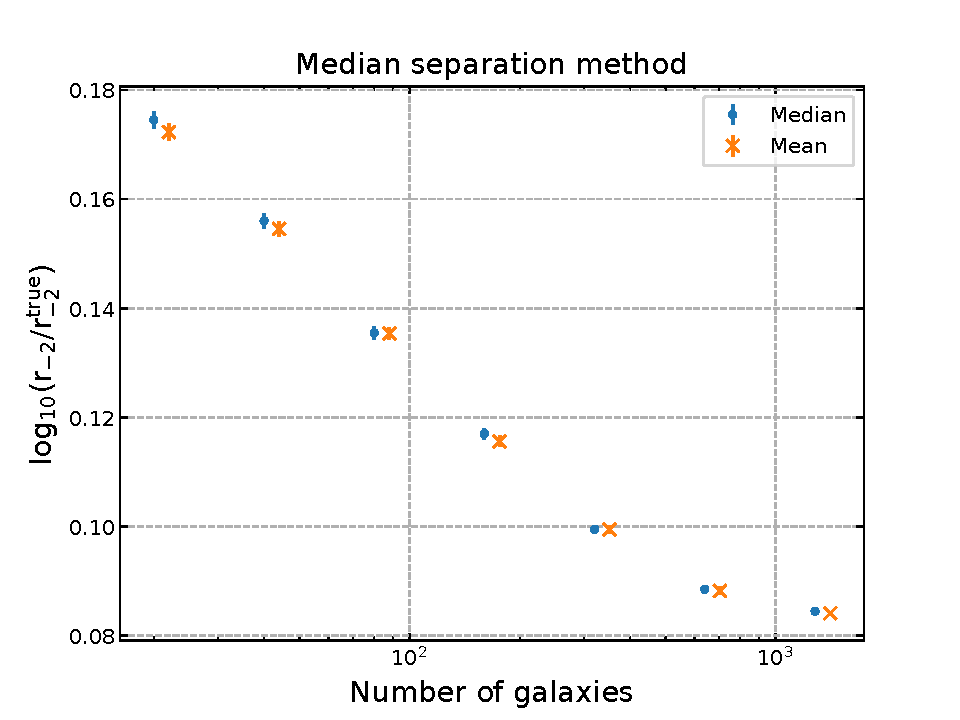
\includegraphics[scale=0.48]{mediansep.pdf}}
		\quad
		\subfloat[Dispersion sur le logarithme du rayon caractéristique. Comme pour le biais on remarque que la dispersion diminue avec le nombre croissant de galaxies.]{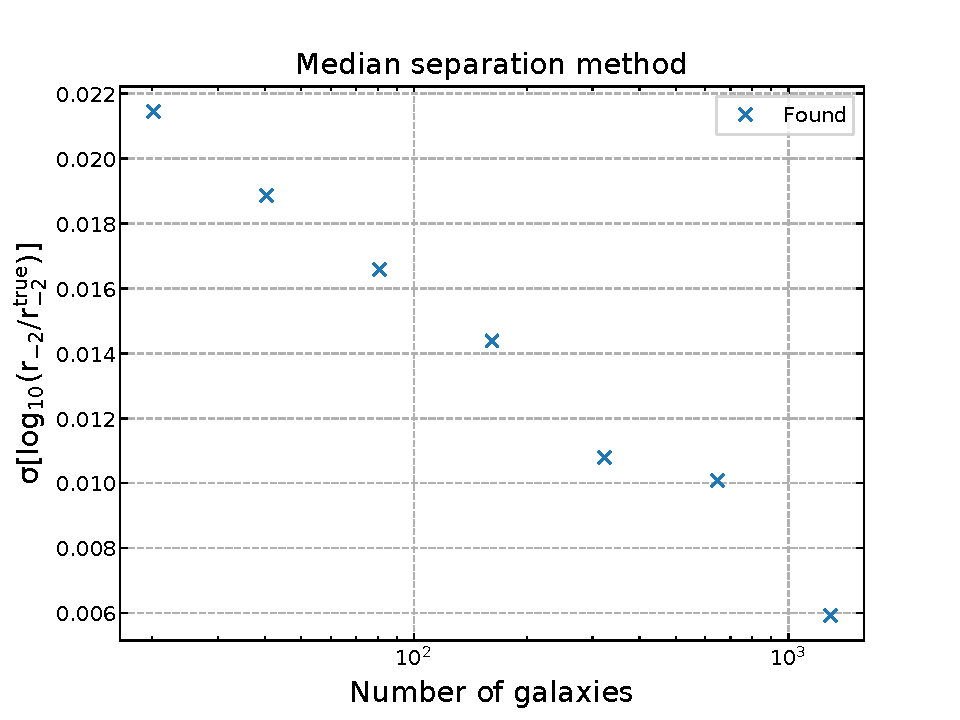
\includegraphics[scale=0.48]{medsep_scat.pdf}}
	\end{center}
	\caption{Biais et dispersion pour la séparation médiane. Chaque valeurs est calculée pour 100 itérations d'amas d'Emmanuel ARTIS contenant 20, 40, 80, 160, 320, 640 et 1280 galaxies.}
	\label{fig:Median}
\end{figure}

\begin{multicols}{2}
  \section{Séparation médiane}
    En plus des méthodes d'optimisation par maximum de vraisemblance on peut obtenir des résultats similaires en considérant cette fois la séparation médiane entre les galaxies.\newline
    Si l'on possède un ensemble de N galaxies alors on aura $N(N-1)/2$ séparations du type $\Delta l_{kl} = \vert l_k - l_l \vert$. On obtient alors une matrice symétrique sur laquelle on peut calculer la séparation médiane sur la partie triangulaire haute par exemple.\newline
Comme on peut le voir sur la Figure \ref{fig:Median} la méthode fournit des résultats corrects avec une erreur relative de l'ordre de $20\%$ lorsqu'on approche $10^3$ galaxies par amas.
  \newpage
  
  \section{Halo de matière noire : Profil NFW et surface de densité}
  \subsection{Profils NFW et NFW tronqués}
    Vers la fin des années 1990 Navarro, Frenck et White montrèrent à l'aide de simulations numériques à N-corps que les halos de matière noire formés dans des cosmogonies de type CDM possèdent deux caractéristiques universelles:
    
    \begin{itemize}
      \item ils suivent tous un profil de densité NFW
      \item ils sont isotropes
    \end{itemize}

    La seconde propriété n'est cependant vraie que dans le cas de halos de matière noire sphériques. Le profil NFW est généralement écrit sous la forme\cite{NFW1996}
    
    \begin{equation}
      \label{NFW_profile}
      \frac{\rho(r)}{\rho_{crit}} = \frac{\delta_{crit}}{(r/r_s) ( 1 + r / r_s)^2}
    \end{equation}
    
    Où $r_s$ représente le rayon de pente -2 et $\delta_{char}$ est une surdensité caractéristique que l'on relie au paramètre de concentration $c = r_s / r_v$ via la formule\cite{Mo_concentration}
    
    \begin{equation}
      \delta_{char} = \frac{200}{3} \frac{c^3}{\ln(1+c) - c / (1+c)}
    \end{equation}
    
  \subsection{Densité surfacique projetée}
    Bien que la distribution spatiale 3D soit utile à connaître, la véritable quantité que l'on peut comparer aux données n'est pas la densité mais la densité surfacique projetée sur le ciel. Celle-ci est obtenue en intégrant le profil de densité le long de la ligne de visée
    
    \begin{equation}
      \Sigma (R) = \int_{\mathbb{R}} \rho (r) dz
    \end{equation}
    
    Où $r$ est le rayon physique et $z$ est la composante selon la ligne de visée. En notant $R$ le rayon dans le plan du ciel, on peut réécrire cette dernière équation comme
    
    \begin{equation}
      \label{Surface_density}
      \Sigma(R) = 2 \int _{R}^{\infty} \frac{r \rho (r) dr}{(r^2 - R^2)^{1/2}} 
    \end{equation}
    
    Cette équation possède une solution analytique utilisée par PROF-CL pour le calcul du likelihood et dont la formule est fournie en annexe. Dans le cas d'un modèle NFW tronqué l'équation (\ref{Surface_density}) reste identique et on a seulement le changement $\infty \rightarrow R_t$ au niveau de la borne supérieure. Dans ce cas il existe aussi une solution analytique fournie en annexe.

  \newpage
  \section{Calcul du log-likelihood}
  \subsection{Maximum de vraissemblance appliqué aux amas de galaxies}
    Jusque dans les années 1980 l'unique méthode permettant de déterminer les propriétés des amas de galaxies tel que leur distribution radiale de masse était une méthode de type binning-fitting. Les images étaient découpés en anneaux de taille arbitraire et le nombre de galaxies était compté dans chaque anneaux. Sarazzin montra\cite{Sarazin1980} que ce type de méthode faisait apparaître un bias lié au choix de la taille des anneaux et que la taille caractéristique des amas pouvait significativement changer d'une étude à l'autre de par ce simple biais. Il proposa une méthode sans binning basé sur le principe de \textbf{maximum de vraissemblance} (nommé par la suite likelihood).\newline
    L'idée est à présent d'assigner à chaque galaxie une probabilité de la trouver dans sa position étant donné le modèle considéré et les paramètres testés, puis de construire le likelihood comme le produit de ces probabilités. Pour un ensemble de N galaxies de positions $ \lbrace X_i = (x_i , y_i )_{1 < i < N} \rbrace $, en notant $\theta$ l'ensemble des paramètres testés on peut écrire le likelihood comme
    
    \begin{equation}
      \label{Likelihood}
      \mathscr{L} = \prod_{i=1}^N p( X_i | \theta)
    \end{equation}
    
    Par la suite, $p(X_i | \theta)$ ne représentera pas directement une probabilité mais une densité de probabilité dont l'intégrale sur l'ensemble des paramètres est normalisée à 1. Pour des raisons pratiques, les probabilités étant en réalité très faibles, on préférera travailler sur le logarithme du likelihood (par la suite appelé log-likelihood). Enfin puisqu'il semble plus facile de minimiser une fonction que de la maximiser on travaillera sur l'opposé du log-likelihood qui se note à présent
    
    \begin{equation}
      \label{Log_Likelihood}
      - \log \mathscr{L} = - \sum_{i=1}^N p (X_i \in cluster) \log p (X_i | \theta)
    \end{equation}
    
    Où on a pris soin de pondérer chaque terme par une probabilité de trouver chaque galaxie dans l'amas correspondant (fournie pour les amas d'AMICO). Si la probabilité d'appartenance des galaxies à l'amas considéré n'est pas connue, on la prend à 1.
    
    \subsection{Calcul de la probabilité}
    Soit $\theta$ l'ensemble des paramètres considérés et $ X_i = (x_i , y_i)$ l'ensemble des positions des galaxies. Lors du calcul de la vraisemblance il faut pouvoir attribuer une probabilité $p(X_i | \theta)$ pour chaque galaxie de la trouver dans la configuration considérée étant donnés les paramètres testés.
La probabilité de trouver une galaxies à une distance R du centre dans un modèle à symétrie sphérique avec fond est donnée par\cite{Mamon2010}
    \begin{equation}
      \label{Prob_uv}
      p(R | \theta) =  \frac{2\pi R [ \Sigma (R ; \theta ) + \Sigma_{bg} ]}{N_{tot}}
    \end{equation}
    Où $\Sigma$ et $\Sigma_{bg}$ représentent respectivement la densité surfacique du modèle et du fond (que l'on considérera constant). Pour un amas dont l'extension angulaire va de $R_{min}$ à $R_{max}$ on écriera le nombre total de galaxies comme la somme de la contribution de l'amas projeté $N_p$ et du fond, i.e.
    \begin{equation}
      \label{N_tot}
      \begin{split}
        N_{tot} =  & N_p (R_{max} ; \theta) - N_p (R_{min} ; \theta) \\
                   & + \pi \Sigma_{bg} (R_{max}^2 - R_{min}^2 )
      \end{split}
    \end{equation}

  En pratique le terme $2\pi R$ n'est rien d'autre qu'un vecteur de composantes constantes qui n'interviendra pas dans la procédure de minimization. On peut donc se permettre de ne pas le calculer (en gardant à l'esprit que les probabilités ne sont plus normalisées).\newline
  Calculer le log-likelihood revient donc en principe à calculer la densité surfacique du modèle.
  
  \newpage
  \section{Méthodes de minimization : étude et amélioration de leur efficacité}
  \subsection{Méthodes}
  
\end{multicols}
\newpage
\bibliography{ref}
\bibliographystyle{ieeetr}

\newpage
\appendix
\section{Solutions analytiques de la densité de surface NFW/NFW tronqué}
Dans le cas d'un profil NFW, la densité surfacique donnée par la solution de l'équation (\ref{Surface_density}) vaut\cite{Lokas2001}

  \begin{equation}
    test  
  \end{equation}
\end{document}
